\documentclass[border=4pt,12pt]{standalone}
% House style for redrawn exam diagrams (diagram-v4: 0.4pt lines, filled -latex arrows, fine dashes; stipple and hatching drawn as real dots/lines (no PDF/SVG patterns, so they render in every browser and at any scale); transparent background). Every figure \input's this.
\usepackage{amsmath,amssymb}
\usepackage{txfonts}
\usepackage{pdfrender,xcolor}
% \halo{text}: label on shading. The shading stops just around each letter's outline (a thin knock-out that follows the
% glyphs, like the papers' typesetting), never a box. Owner: "I don't want a box around the text".
\newcommand{\halo}[1]{\leavevmode\rlap{\pdfrender{TextRenderingMode=2,LineWidth=2.2pt,LineJoinStyle=1,StrokeColor=white,FillColor=white}#1}#1}
\usepackage{tikz,pgfplots}
\pgfplotsset{compat=1.18}
\usetikzlibrary{arrows.meta,calc,angles,quotes,patterns,patterns.meta,intersections,positioning,decorations.markings,shapes.geometric}
% Stipple and hatching are drawn as actual dots / lines clipped to the region (path picture), NOT as pattern fills:
% SVG <pattern> fills vanish or blur when browsers scale the image, so the owner could not see the shading.
% Each dot is a 0.72pt square (keeps SVGs small; reads as a dot at print size). Dots sit on one global staggered grid, so neighbouring regions line up.
\makeatletter
\newdimen\ex@x \newdimen\ex@y \newdimen\ex@xa \newdimen\ex@ya \newdimen\ex@xb \newdimen\ex@yb \newcount\ex@row
\def\exam@stipplecolor{black!75}\def\exam@dotr{0.42pt}\def\exam@dotgap{2.5}
\def\ex@rowdots{\ifdim\ex@x<\ex@xb \pgfpathrectangle{\pgfqpoint{\dimexpr\ex@x-0.36pt\relax}{\dimexpr\ex@y-0.36pt\relax}}{\pgfqpoint{0.72pt}{0.72pt}}\advance\ex@x by \exam@dotgap pt\relax\expandafter\ex@rowdots\fi}
\def\exam@stipple{%
  \pgftransformreset% dots are sized in real points even inside scaled pictures
  \pgfpointanchor{path picture bounding box}{south west}\ex@xa=\pgf@x \ex@ya=\pgf@y
  \pgfpointanchor{path picture bounding box}{north east}\ex@xb=\pgf@x \ex@yb=\pgf@y
  \pgfsetfillcolor{\exam@stipplecolor}\pgfmathsetmacro\ex@h{\exam@dotgap/2}%
  \pgfmathtruncatemacro\ex@r{floor(\ex@ya/\ex@h)-1}\ex@row=\ex@r\relax
  \ex@y=\ex@r\dimexpr\ex@h pt\relax
  \loop\ifdim\ex@y<\ex@yb
    \pgfmathtruncatemacro\ex@c{floor(\ex@xa/\exam@dotgap)-1}\ex@x=\ex@c\dimexpr\exam@dotgap pt\relax
    \ifodd\ex@row \advance\ex@x by \ex@h pt\fi
    \ex@rowdots
    \advance\ex@y by \ex@h pt \advance\ex@row by 1
    \ifnum\numexpr\ex@row-(\ex@row/4)*4\relax=0 \pgfusepath{fill}\fi% flush every 4 rows: bounded TeX memory, few clip copies in the SVG
  \repeat\pgfusepath{fill}}
\newdimen\ex@d
\def\exam@hatch#1{% #1 = 1 for /, -1 for \ ; lines 45 degrees, 3pt apart
  \pgftransformreset
  \pgfpointanchor{path picture bounding box}{south west}\ex@xa=\pgf@x \ex@ya=\pgf@y
  \pgfpointanchor{path picture bounding box}{north east}\ex@xb=\pgf@x \ex@yb=\pgf@y
  \ex@d=\dimexpr\ex@yb-\ex@ya\relax \ex@x=\dimexpr\ex@xa-\ex@d\relax
  \loop\ifdim\ex@x<\ex@xb
    \ifnum#1>0 \pgfpathmoveto{\pgfqpoint{\ex@x}{\ex@ya}}\pgfpathlineto{\pgfqpoint{\dimexpr\ex@x+\ex@d\relax}{\ex@yb}}%
    \else \pgfpathmoveto{\pgfqpoint{\ex@x}{\ex@yb}}\pgfpathlineto{\pgfqpoint{\dimexpr\ex@x+\ex@d\relax}{\ex@ya}}\fi
    \advance\ex@x by 4.24pt
  \repeat
  \pgfsetlinewidth{0.4pt}\pgfsetstrokecolor{black}\pgfusepath{stroke}}
\def\examstipple{\exam@stipple}\def\examhatch{\exam@hatch}\def\examsetstipplecolor#1{\def\exam@stipplecolor{#1}}\def\examsetdotgap#1{\def\exam@dotgap{#1}}
\makeatother
% (legacy pattern kept for old files)
% staggered stipple like the NESA papers' dotted shading
\pgfdeclarepatternformonly{exam stipple}{\pgfpointorigin}{\pgfqpoint{2.2pt}{2.2pt}}{\pgfqpoint{2.2pt}{2.2pt}}{%
  \pgfpathcircle{\pgfqpoint{0.55pt}{0.55pt}}{0.42pt}\pgfpathcircle{\pgfqpoint{1.65pt}{1.65pt}}{0.42pt}\pgfusepath{fill}}
\tikzset{
  every picture/.style={line width=0.6pt, >={Latex[length=2mm,width=1.3mm]}},
  curve/.style={line width=0.6pt},
  open arrow/.style={-{Latex[length=2mm,width=1.3mm]}},  % owner: filled -latex heads everywhere, no open chevrons
  aux/.style={dash pattern=on 2pt off 1.5pt, line width=0.6pt},
  shade/.code={\def\exA{#1}\def\exB{none}\ifx\exA\exB\else\pgfkeysalso{fill=black!18}\fi},
  shade/.default=on,
  shade dots/.style={fill=none, path picture={\examstipple}},
  stipple color/.code={\examsetstipplecolor{#1}},
  stipple gap/.code={\examsetdotgap{#1}},
  shade dense dots/.style={fill=none, stipple gap=1.6, path picture={\examstipple}},
  shade hatch/.style={fill=none, path picture={\examhatch{1}}},
  shade hatch reverse/.style={fill=none, path picture={\examhatch{-1}}},
  shade solid/.style={fill=black},
  pt/.style={circle, fill, inner sep=1.1pt},
  open pt/.style={circle, draw, fill=white, inner sep=1.1pt},
}
\pgfplotsset{
  exam axes/.style={axis lines=middle, axis line style={->}, xlabel={$x$}, ylabel={$y$},
    xlabel style={anchor=west}, ylabel style={anchor=south}, tick label style={font=\small},
    every axis plot/.append style={line width=0.6pt, black}, samples=200, clip=false,
    enlargelimits=false, axis on top},
}

\begin{document}
% crop pixels: x=311.6+47.35u, y=380-83.6v; curve traced from the crop
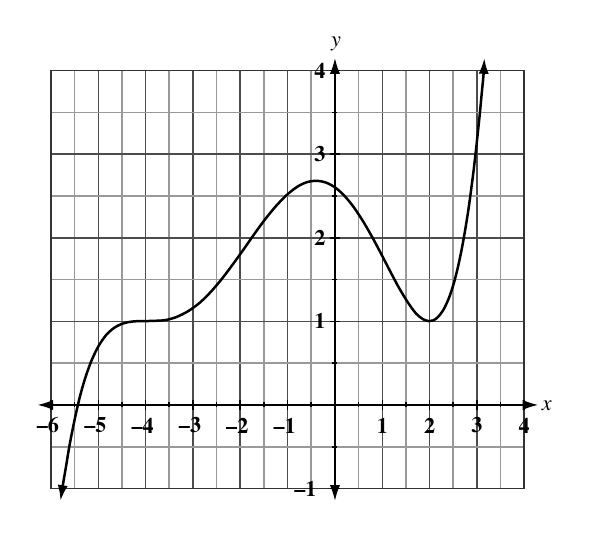
\begin{tikzpicture}[x=0.0127cm,y=-0.0127cm,every node/.style={font=\fontsize{8}{9.6}\selectfont}]
\draw[black!70] (27.5,463.6) -- (27.5,45.6);
\draw[black!40] (51.2,463.6) -- (51.2,45.6);
\draw[black!70] (74.9,463.6) -- (74.9,45.6);
\draw[black!40] (98.5,463.6) -- (98.5,45.6);
\draw[black!70] (122.2,463.6) -- (122.2,45.6);
\draw[black!40] (145.9,463.6) -- (145.9,45.6);
\draw[black!70] (169.6,463.6) -- (169.6,45.6);
\draw[black!40] (193.2,463.6) -- (193.2,45.6);
\draw[black!70] (216.9,463.6) -- (216.9,45.6);
\draw[black!40] (240.6,463.6) -- (240.6,45.6);
\draw[black!70] (264.2,463.6) -- (264.2,45.6);
\draw[black!40] (287.9,463.6) -- (287.9,45.6);
\draw[black!40] (335.3,463.6) -- (335.3,45.6);
\draw[black!70] (359.0,463.6) -- (359.0,45.6);
\draw[black!40] (382.6,463.6) -- (382.6,45.6);
\draw[black!70] (406.3,463.6) -- (406.3,45.6);
\draw[black!40] (430.0,463.6) -- (430.0,45.6);
\draw[black!70] (453.7,463.6) -- (453.7,45.6);
\draw[black!40] (477.3,463.6) -- (477.3,45.6);
\draw[black!70] (501.0,463.6) -- (501.0,45.6);
\draw[black!70] (27.5,463.6) -- (501.0,463.6);
\draw[black!40] (27.5,421.8) -- (501.0,421.8);
\draw[black!40] (27.5,338.2) -- (501.0,338.2);
\draw[black!70] (27.5,296.4) -- (501.0,296.4);
\draw[black!40] (27.5,254.6) -- (501.0,254.6);
\draw[black!70] (27.5,212.8) -- (501.0,212.8);
\draw[black!40] (27.5,171.0) -- (501.0,171.0);
\draw[black!70] (27.5,129.2) -- (501.0,129.2);
\draw[black!40] (27.5,87.4) -- (501.0,87.4);
\draw[black!70] (27.5,45.6) -- (501.0,45.6);
\draw[black!80] (27.5,463.6) rectangle (501.0,45.6);
\draw[<->] (14,380) -- (515,380);
\draw[<->] (311.6,33) -- (311.6,476);
\draw (27.5,375) -- (27.5,385);\draw (51.2,377.5) -- (51.2,382.5);\draw (74.9,375) -- (74.9,385);\draw (98.5,377.5) -- (98.5,382.5);\draw (122.2,375) -- (122.2,385);\draw (145.9,377.5) -- (145.9,382.5);\draw (169.6,375) -- (169.6,385);\draw (193.2,377.5) -- (193.2,382.5);\draw (216.9,375) -- (216.9,385);\draw (240.6,377.5) -- (240.6,382.5);\draw (264.2,375) -- (264.2,385);\draw (287.9,377.5) -- (287.9,382.5);\draw (335.3,377.5) -- (335.3,382.5);\draw (359.0,375) -- (359.0,385);\draw (382.6,377.5) -- (382.6,382.5);\draw (406.3,375) -- (406.3,385);\draw (430.0,377.5) -- (430.0,382.5);\draw (453.7,375) -- (453.7,385);\draw (477.3,377.5) -- (477.3,382.5);\draw (501.0,375) -- (501.0,385);\draw (306.6,463.6) -- (316.6,463.6);\draw (309.1,421.8) -- (314.1,421.8);\draw (309.1,338.2) -- (314.1,338.2);\draw (306.6,296.4) -- (316.6,296.4);\draw (309.1,254.6) -- (314.1,254.6);\draw (306.6,212.8) -- (316.6,212.8);\draw (309.1,171.0) -- (314.1,171.0);\draw (306.6,129.2) -- (316.6,129.2);\draw (309.1,87.4) -- (314.1,87.4);\draw (306.6,45.6) -- (316.6,45.6);
\draw[<->, line width=0.9pt] plot[smooth] coordinates {(37,476) (39.51,459.5) (42.6,441.4) (45.63,422.8) (49.21,404.2) (53.2,385.4) (57.47,367.8) (62.61,350.5) (68.45,334.7) (75.28,320.8) (82.54,310.3) (90.39,303.1) (99.52,298.5) (110.6,296.4) (127,296) (141.3,295.2) (152.9,292.1) (164.9,286.1) (176.4,277.7) (187.4,266.9) (198.6,253.7) (209.7,239) (220.9,223.4) (232,207.5) (242.8,192.9) (253.9,179.6) (265,168.5) (275.4,160.8) (284.8,156.8) (293.9,155.8) (302.5,157.5) (311.7,162.4) (321.1,170.8) (330.7,182.6) (340.1,196.9) (349.2,212.7) (358.1,229.4) (367.1,246.8) (375.8,263.1) (384.9,278) (393,288.9) (399.8,294.3) (405.3,296.1) (409.5,295.6) (414,292.7) (419.8,285.4) (425.7,272.8) (430.8,257.3) (435.1,240) (438.9,221.6) (442.2,203) (445.2,184) (447.8,164.9) (450.3,145.5) (452.5,126.4) (454.6,107) (456.6,87.82) (458.4,68.61) (460.2,49.85) (461,33)};
\node at (24.5,400.5) {\textbf{\textendash6}};
\node at (71.9,400.5) {\textbf{\textendash5}};
\node at (119.2,400.5) {\textbf{\textendash4}};
\node at (166.6,400.5) {\textbf{\textendash3}};
\node at (213.9,400.5) {\textbf{\textendash2}};
\node at (261.2,400.5) {\textbf{\textendash1}};
\node at (359.0,400.5) {\textbf{1}};
\node at (406.3,400.5) {\textbf{2}};
\node at (453.7,400.5) {\textbf{3}};
\node at (501.0,400.5) {\textbf{4}};
\node at (296.6,296.4) {\textbf{1}};
\node at (296.6,212.8) {\textbf{2}};
\node at (296.6,129.2) {\textbf{3}};
\node at (296.6,45.6) {\textbf{4}};
\node[anchor=east] at (303.1,463.6) {\textbf{\textendash1}};
\node at (523,381) {$x$};\node at (312.6,19) {$y$};
\end{tikzpicture}
\end{document}
